% !TEX root = ../main.tex
\section{When Does TSGD Shine?}
\label{sec:when-tsgd-shines}

The distinction between noise magnitude and noise variation is easiest
to see on simple objectives. We compare the expected squared true
gradient $G_k:=\mathbb E[\|\nabla f(x_k)\|^2]$, keeping track of the
initial estimate as a separate resource.

\subsection{Accurate Differences Despite Noisy Gradients}
\label{subsec:additive-noise-comparison}

Consider $f(x)=x^2/2$ and an unbiased oracle $h(x,\xi)=x+\xi$,
where $\mathbb E[\xi]=0$ and $\mathbb E[\xi^2]=\sigma^2$.
The individual gradients can be arbitrarily noisy, yet
\[
h(x,\xi)-h(y,\xi)=x-y=\nabla f(x)-\nabla f(y).
\]
Thus $\delta=0$, independently of $\sigma$. With exact
initialization, TSGD follows gradient descent exactly. From $x_0=1$
with $\eta=1$, it reaches the minimizer in one step. SGD instead
has $x_{k+1}=-\xi_k$ and $G_k=\sigma^2$ for every $k\geq1$.
Horizon-dependent steps can remove this SGD residual, but do not
recover the noiseless trajectory; the exact calculations are in
Appendix~\ref{app:additive-details}. Accurate initialization is
essential here: exact transport preserves any initial error.

\subsection{Fixed Noise Magnitude, Variable Similarity}
\label{subsec:fixed-variance-variable-similarity}

To vary similarity without changing the noise magnitude, take
\begin{equation}
\label{eq:fixed-variance-oracle}
f(x)=\frac L2x^2,\qquad
h(x,\varphi)=Lx+\sqrt2\sigma\cos(\omega x+\varphi),
\qquad \varphi\sim\operatorname{Unif}[0,2\pi).
\end{equation}
Each new sample is an independent phase; a transport difference
uses the same phase at both endpoints. For the noise
$r(x,\varphi)=h(x,\varphi)-Lx$,
\begin{equation}
\label{eq:phase-noise-moments}
\mathbb E[r(x,\varphi)^2]=\sigma^2,\qquad
\mathbb E[|r(x,\varphi)-r(y,\varphi)|^2]
=4\sigma^2\sin^2\!\left(\frac{\omega(x-y)}2\right).
\end{equation}
The smallest global similarity constant is $\delta=\sigma\omega$
(Appendix~\ref{app:sinusoidal-proof}). Pointwise noise has the same
distribution for every $x$ and $\omega$, so SGD has identical
expected squared-gradient dynamics at every frequency. TSGD,
however, sees exact differences at $\omega=0$ and increasingly
permissive similarity bounds as $\omega$ increases. Its actual
transport error depends on the displacement through the sine term.

\begin{figure}[t]
\centering
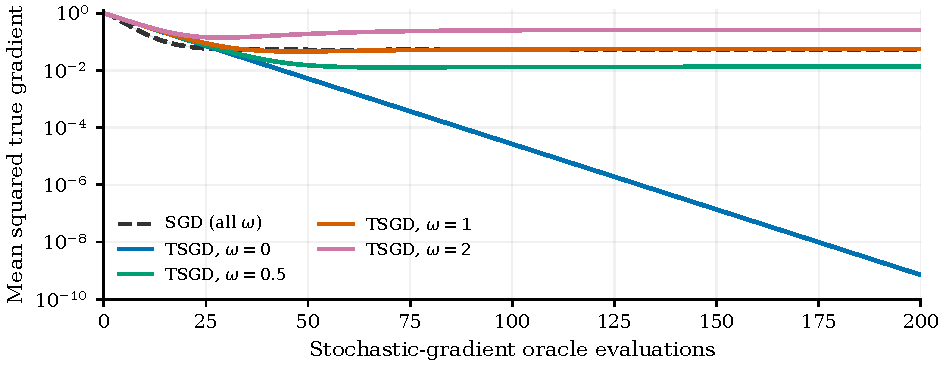
\includegraphics[width=\linewidth]{figures/similarity_experiment.pdf}
\caption{Same pointwise variance, different transport accuracy.
Monte Carlo means over $10^5$ runs, with bands of two standard errors;
$L=\sigma=x_0=1$ and a common constant stepsize $\eta=0.1$.
Every method starts from the same exact estimate, obtained using two
antithetic oracle evaluations, charged on the horizontal axis.
Subsequent SGD updates cost one evaluation and TSGD updates cost two.
SGD is simulated at $\omega=1$; its expected curve is identical at
all frequencies. Appendix~\ref{app:numerical-details} gives the
sampling, cost accounting, and reproducible numerical details.}
\label{fig:similarity-experiment}
\end{figure}

Figure~\ref{fig:similarity-experiment} isolates this distinction at
equal oracle cost. At small frequencies, TSGD retains accurate
information despite the persistent pointwise noise. At $\omega=2$,
its mean squared true-gradient norm exceeds SGD's in these runs. The figure shows
why noise magnitude alone cannot predict the usefulness of
transport; it does not assert monotonicity of each realized error
with frequency or superiority under every stepsize choice.

\subsection{When Fresh Gradients Are Preferable}
\label{subsec:multiplicative-noise-comparison}

Now let
\begin{equation}
\label{eq:multiplicative-comparison-oracle}
f(x)=\frac{x^2}{2},\qquad h(x,a)=ax,\qquad
\mathbb P(a=0)=\mathbb P(a=2)=\frac12,\qquad x_0=1.
\end{equation}
Here the gradient-noise variance is $x^2$: fresh gradients become
exact at the minimizer, although global BV fails. Similarity holds
with $\delta=1$. At the common stepsize $\eta=1/2$, each SGD sample
either leaves the iterate unchanged or sends it to zero, so
$G_k^{\mathrm{SGD}}=2^{-k}$. In contrast, exactly initialized TSGD
satisfies $g_{k+1}=(1-a_{k+1}/2)g_k$. Its estimator becomes zero at
the first sample $a_{k+1}=2$, wherever the iterate happens to be.
The exact calculation in Appendix~\ref{app:multiplicative-details}
gives
\[
g_k\longrightarrow0\quad\text{almost surely},\qquad
G_k^{\mathrm{TSGD}}\longrightarrow\frac12.
\]
This is false convergence: a vanishing estimate need not indicate
a vanishing true gradient. Fresh information can therefore be
preferable even when initialization is exact.

\subsection{What Transport Cannot Do}
\label{subsec:four-case-summary}

The two sources of error in Section~\ref{subsec:martingale-interpretation}
also interact. In the quadratic model
$f(x)=\lambda x^2/2$, $h(x;a,b)=(\lambda+a)x+b$, with $\lambda>0$, take independent
centered $a,b$ with $\mathbb E[a^2]=\delta^2$. Coupling cancels $b$;
initialization and the remaining transport noise produce the four
regimes in Table~\ref{tab:four-error-regimes}.

\begin{table}[t]
\centering
\small
\begin{tabular}{@{}lcc@{}}
\toprule
Initialization & Exact transport & Stochastic transport\\
\midrule
Exact & Gradient descent & Accumulated transport error\\
Inexact & Persistent initial error & Both errors and their interaction\\
\bottomrule
\end{tabular}
\caption{Four regimes in the quadratic model, with a stable constant
stepsize. The exact-transport identities also hold for general
objectives; the explicit limiting errors and stability condition
are established in Appendix~\ref{app:quadratic-dynamics}.}
\label{tab:four-error-regimes}
\end{table}

Exact differences cannot identify a missing constant gradient
offset: adding $\langle c,x\rangle$ to an objective leaves every
gradient difference unchanged. An initial error $e_0$ therefore
persists under exact transport, and TSGD follows GD on
$f(x)+\langle e_0,x\rangle$. With stochastic transport, even exact
initialization can lead to false convergence, as above. A noisy
initial estimate also changes the early displacements, and hence
the transport errors subsequently accumulated. These limitations
explain why similarity and initialization accuracy enter the
convergence theory separately.
